\documentclass{subfiles}

\begin{document}
    \marginnote{\textbf{\textit{VL 10}}\\16.05.2023, 11:45}[-0.5cm]
    \subsubsection*{Das Fourierbild}

    \subsubsection*{Ergebnis}
    Mit der obigen Aufgabe folgt dann, daß der Impuls $p$ über die Zeit nicht erhalten ist; also $\overline p\neq p$ und in der Sprache des Kommutators $[p,H]\neq 0$. Optisch erhalten wir für die Wahrscheinlichkeitsverteilung eine \emph{Aufspaltung} in zwei Peaks; Das Teilchen selbst ist allerdings nicht aufgespalten - die Implikation an dieser Stelle gilt also nicht. 
    \begin{figure}[H]
        \centering
        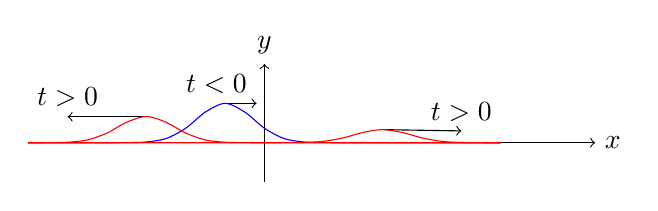
\begin{tikzpicture}
            \draw[->] (-3, 0) -- (4.2, 0) node[right] {$x$};
            \draw[->] (0, -0.5) -- (0, 1) node[above] {$y$};

            \draw[->] (-1.5, 0.33) -- (-2.5, 0.33) node[above] {$t>0$};
            \draw[->] (1.5, 0.166) -- (2.5, 0.15) node[above] {$t>0$};
            \draw[->] (-0.5,0.5) -- (-0.1,0.5) node[above left] {$t<0$};

            \draw[scale=0.5, domain=-6:6, smooth, variable=\x, blue] plot ({\x}, {exp(-(\x + 1)^2)});
            \draw[scale=0.5, domain=-6:6, smooth, variable=\x, red]  plot ({\x}, {exp(-(\x - 3)^2) / 3});
            \draw[scale=0.5, domain=-6:6, smooth, variable=\x, red]  plot ({\x}, {2 * exp(-(\x + 3)^2) / 3});
        \end{tikzpicture}
        \caption{Wahrscheinlichkeitsverteilung zu $t<0$ (blau) und $t>0$ (rot).}
    \end{figure}
    Beachtlich ist nun, daß das quantenmechanische Teilchen mit einer Wahrscheinlichkeit $>0$ auf der rechten Seite der Potentialbarriere vorfindbar ist; dies ist Resultat der Heisenbergschen Unschärferelation:
    \[\var_\psi(Q)\cdot\var_\psi(H)\geq \frac{1}{2}\abs{\langle[H,x]\rangle_{\psi}}\qquad \bbbra{= \frac{\hbar\cdot\langle p\rangle_{u_{\exp,0}}}{2\cdot m}\neq 0}.\]
    Daraus folgt für eine Varianz $\var_\psi(Q)>0$ eine Varianz $\var_{\psi}(H) \approx p^2/(2m)$, sodaß $\hbar/\overline p = 1/\kappa$. 
    

\end{document}